\documentclass[tikz,border=6pt]{standalone}
\usepackage{amsmath}
\usetikzlibrary{calc}

\begin{document}
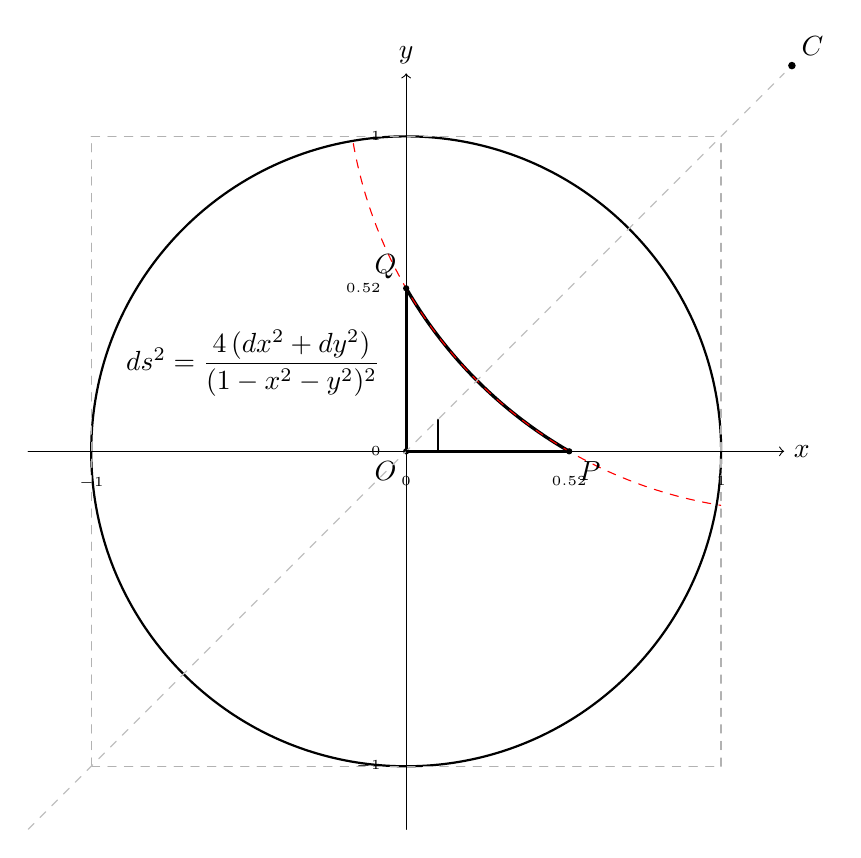
\begin{tikzpicture}[scale=4, line cap=round, line join=round]
  % Parameters
  \pgfmathsetmacro{\a}{sqrt(2 - sqrt(3))} % a ~ 0.5176
  \pgfmathsetmacro{\h}{( (\a*\a) + 1 ) / (2*\a)} % h = (a^2+1)/(2a)
  \pgfmathsetmacro{\R}{sqrt(2*\h*\h - 1)} % R = sqrt(h^2+h^2 - 1)
  
  % Points
  \coordinate (O) at (0,0);
  \coordinate (P) at (\a,0);
  \coordinate (Q) at (0,\a);
  \coordinate (C) at (\h,\h);
  
  % Angles to draw arc around C from P to Q
  \pgfmathsetmacro{\angP}{atan2(0-\h, \a-\h)} % angle of CP vector (degrees)
  \pgfmathsetmacro{\angQ}{atan2(\a-\h, 0-\h)} % angle of CQ vector (degrees)

  % Unit circle (boundary)
  \draw[thick] (0,0) circle (1);

  % Axes and Grid
  \draw[gray!60,dashed,thin] (-1,-1) grid (1,1);
  \draw[->] (-1.2,0) -- (1.2,0) node[right] {$x$};
  \draw[->] (0,-1.2) -- (0,1.2) node[above] {$y$};

  % Ticks
  \foreach \x in {-1,0,1}
    \node[below,yshift=-2mm,font=\tiny] at (\x,0) {\pgfmathprintnumber{\x}};
  \foreach \y in {-1,0,1}
    \node[left,xshift=-2mm,font=\tiny] at (0,\y) {\pgfmathprintnumber{\y}};

  % Tick labels for P and Q
  \pgfmathsetmacro{\pCoord}{\a}
  \node[below,yshift=-2mm,font=\tiny] at (P) {\pgfmathprintnumber{\pCoord}};
  \pgfmathsetmacro{\qCoord}{\a}
  \node[left,xshift=-2mm,font=\tiny] at (Q) {\pgfmathprintnumber{\qCoord}};
  
  % Metric text
  \node[anchor=west] at (-0.92,0.28) {$ds^2=\dfrac{4\,(dx^2+dy^2)}{(1-x^2-y^2)^2}$};
  
  % Geodesic triangle: OP and OQ (diameters)
  \draw[very thick] (O) -- (P);
  \draw[very thick] (O) -- (Q);
  
  % Geodesic arc PQ: circle centered at C, orthogonal to boundary
  \draw[very thick] ($(C)+({\R*cos(\angP)},{\R*sin(\angP)})$) arc[start angle=\angP, end angle=\angQ, radius=\R];
  
  % Added full circle from C with radius CP, clipped to unit square
  \begin{scope}
    \clip (-1,-1) rectangle (1,1);
    \draw[red,dashed,thin] (C) circle (\R);
  \end{scope}
  
  % Points
  \fill (O) circle (0.01);
  \fill (P) circle (0.01);
  \fill (Q) circle (0.01);
  \fill (C) circle (0.012); % emphasize C
  
  % Labels
  \node[below left] at (O) {$O$};
  \node[below right] at (P) {$P$};
  \node[above left] at (Q) {$Q$};
  \node[above right] at (C) {$C$};
  
  % Diagonal y=x (faint guide to show C lies on it)
  \draw[gray!50,dashed] (-1.2,-1.2) -- (1.2,1.2);
  
  % Indicate right angle at QOP
  \draw[thick] (O) -- ++(0.1,0) -- ++(0,0.1); % Right angle mark at O
\end{tikzpicture}
\end{document}